\section{The pKa closure: full construction, measured sweep, and trained comparison}
\label{sec:si-pka}
This section gives the full construction behind \S\ref{sec:pka}: a fixed
Hammett linear-free-energy relationship (LFER) $g(\hammett)=\mathrm pK_{a,0}-\rho\,\hammett$ over the
Hammett substituent constant $\hammett$ (with $\mathrm pK_{a,0},\rho$ the per-scaffold
Hansch--Leo--Taft reaction-series constants), for which Hansch--Leo tabulated constants provide an
external oracle $\zstar$. The analogy is close: as with the $\sigma$-profile through COSMO-SAC, a
learnable physical descriptor is pushed through a fixed, approximate, differentiable map. The two
classic LFER failure modes fall cleanly onto the two error channels of Lemma~\ref{prop:decomp}:
\emph{resonance saturation}---a curvature in $\hammett$ that the linear closure structurally cannot
represent---is a mis-map of a function of $\zstar$ and lands in $\Bclos$; \emph{ortho/steric} field
effects, absent from the tabulated constants, are information the intermediate lacks and land in
$\Binsuf$. The chemical scope is a fidelity sweep: meta/para monosubstituted benzoic acids, phenols,
and anilinium ions are the near-exact ($\Bclos\!\approx\!0$) regime, ortho
(insufficiency-dominated) and polyfunctional the low-fidelity one.

This decomposition is directly visible before any training. Pushed through the fixed Hammett
closure, $p$-nitrophenol reads $\mathrm pK_a\!\approx\!8.3$ against an experimental $\approx7.1$
(and $p$-nitroaniline overshoots similarly): the linear closure is off by $\sim1$ unit exactly
where through-conjugation ($\sigma_{\mathrm H}^-$) breaks it---$\Bclos$ observed in practice.

A controlled semi-synthetic construction on real tabulated $\hammett$ (known ground-truth
channels) validates the estimator and reproduces the paper's central distinction in this second
closure (Fig.~\ref{fig:pka}). Sweeping closure fidelity with a sufficient intermediate, the
grounding gap $\Ggap$ tracks $\Bclos$ (the plug-in estimate recovers the truth to within a few
percent, e.g.\ $0.20$ vs $0.21$, $0.81$ vs $0.81$), the case where Theorem~\ref{thm:gap}'s
proxy is valid. Sweeping the ortho/steric channel with a \emph{well-specified} closure gives
$\Bclos=0$ at every knob while $\Ggap$ rises with the insufficiency fraction, from $-0.035$ at zero
insufficiency through zero near a fraction of $0.25$ to $+0.34$ at $0.7$: at the three fractions
where it is positive it is positive with $\Bclos$ identically zero, which is the pKa realization of
the conflation that makes $\Ggap$ an indicator rather than a certificate. The two negative points
are the same statement in the other direction---a well-specified closure with a nearly sufficient
intermediate leaves the oracle marginally ahead. The oracle-$\hammett$ pipeline
(scaffold-resolved substituent$\to\hammett$ assignment) and this validation extend directly to real
data. On the OPERA experimental $\mathrm pK_a$ compilation \cite{mansouri2019opera} ($7{,}904$
records under the same net-neutral filter), applying the same decomposition to the fixed Hammett
closure yields a \emph{measured} fidelity sweep. On the clean meta/para series ($n{=}158$) the closure
predicts experimental $\mathrm pK_a$ to RMSE $0.55$, with the closure at the input-insufficiency floor:
the leakage-immune lower bound $\mathrm{MSE}-\Binsuf^{\mathrm{up}}$ is $-0.2$ ($95\%$~CI $[-0.4,-0.0]$),
i.e.\ below zero, as a lower bound on the non-negative $\Bclos$ must sit when the LFER predicts as well
as a flexible within-scaffold regressor. There $\Bclos$ is not separately resolvable and is consistent
with a well-specified closure (per-scaffold systematic offsets $\le0.18$). The ortho/heteroaromatic regime ($n{=}846$)
degrades to RMSE $2.26$, dominated by input insufficiency. Here the pKa latent is a \emph{scalar}
Hammett constant, so---unlike the solubility regime---$\Binsuf$ is estimated \emph{directly} rather
than through a coarsening of the closure's argument (\S\ref{sec:decomp}): a within-scaffold
out-of-fold regression estimator gives $\Binsuf=4.5$
($95\%$~CI $[4.0,5.1]$; $\approx89\%$ of the error---the tabulated $\hammett$ carries no ortho
information, exactly the a-priori channel assignment), leaving a closure misspecification
$\Bclos=0.6$ ($[0.3,0.8]$, a stratified within-scaffold molecule bootstrap). Directly estimated is
not point-identified: the estimator is an out-of-fold residual mean square, which is an upper
estimate of $\Ex[\Var(\mathrm{p}K_a\mid\hammett)]$, so $4.5$ is an upper figure and the $0.6$ it
leaves is a lower one---one-sided in the same direction as everywhere else in this paper, and
narrower only because the scalar latent needs no binning (\S\ref{sec:decomp},
\S\ref{sec:pka}). This is the
near-exact-to-degraded transition, measured rather than asserted. This places the pKa closure near the phase-diagram boundary
in its clean regime. \paragraph{Data quality control (uniform, closure-independent).} The trained runs use the canonical
full OPERA set ($7904$ records). A small number of entries are supplied as pre-ionized microstates---an
$[\mathrm{NH}^+]$-protonated aminopyridine at $\mathrm pK_a=-7.78$, a pyrylium $[\mathrm O^+]$, among
others---inconsistent with a neutral-scaffold Hammett assignment, and they degrade the clean pole
(pyridinium RMSE $0.63\!\to\!3.83$). We drop them with one rule, \emph{net formal charge} $\neq0$,
applied uniformly to both strata. It is closure-independent (it never references the oracle residual,
so it cannot be circular) and keeps net-neutral substituents such as nitro $[\mathrm N^+][\mathrm O^-]{=}\mathrm O$.
This removes $5$ of $163$ meta/para rows (restoring the clean pole to RMSE ${\approx}0.55$) and $352$
of $1198$ ortho rows (leaving $846$; the ortho RMSE is essentially unchanged, so the filter does not
manufacture the sign), for $1004$ Hammett-amenable rows.

\paragraph{Evidence for the flip.} We train the physics arm (encoder $\to\hat\sigma_{\mathrm H}\to$ fixed LFER)
on $K{=}20$ stratified $80/20$-within-scaffold splits---a Bemis--Murcko split collapses the meta/para
pole to two ring systems and is unstable---and record the paired per-molecule error against the
deterministic oracle, per stratum. Meta/para: learned MAE $0.48\pm0.09$ vs oracle $0.315\pm0.07$, gap
$-0.165$, oracle better in $19/20$ splits, $90\%$ CI $[-0.28,-0.04]$. Ortho: learned $0.83\pm0.07$ vs
oracle $1.62\pm0.08$, gap $+0.79$, oracle worse in $20/20$ splits, $90\%$ CI $[+0.57,+0.95]$ (both
intervals from the scaffold-cluster bootstrap).

\paragraph{What the two bootstraps do and do not resolve.} We report the sign statements above rather
than the bootstrap $P$ values, because neither bootstrap here carries the resolution a two-decimal $P$
implies. The cluster unit is the Hammett reaction series, and only $G{=}4$ exist (benzoic acid,
phenol, anilinium, pyridinium): the resampling law then has $\binom{7}{4}{=}35$ distinct outcomes and
a finest atom $(1/4)^4{\approx}0.004$, so the cluster-bootstrap $P(\text{oracle worse}){=}1.00$ on
ortho is exactly the statement that all four series means favour the learned arm, and $P{=}0.004$ on
meta/para that exactly one of them does, the other three favouring the oracle. Read as a sign test on
four units those are $p{=}1/16$ and $p{\approx}0.31$; the interval endpoints quoted above are
percentiles of the same $35$-outcome law and are no finer. This is the same small-$G$ caution applied
on the solubility side (\S\ref{sec:si-tables}), where the $P$ values are likewise read as a coarse
band rather than as two-decimal quantities. The split bootstrap adds nothing independent: the $20$
splits resample train/test assignments over the same molecules (each molecule lands in ${\approx}4$
test sets), so it prices split-to-split noise rather than molecule sampling, and with all $20$ ortho
gaps positive it returns $1.000$ by construction---a restatement of the $20/20$, not a second
confirmation. What the flip rests on is therefore the sign consistency across splits and series and
the size of the ortho gap ($+0.79$ against an oracle MAE of $1.62$, ${\approx}49\%$), not on a $P$
value. A leave-one-series-out refit, the estimate that would settle the series-level question at
$G{=}4$, was not run.

\paragraph{The crossover law and its scope boundary.} A competence sweep (train fraction
$\in\{1.0,0.5,0.25,0.12\}$ and, as the low-competence extreme, scaffold extrapolation; six seeds each)
confirms the sign is set by the crossover of the learned error against the fidelity-fixed oracle
threshold. On meta/para the learned arm rises from $0.46$ to $0.98$ as data shrinks but never reaches
the $0.31$ oracle threshold, so grounding helps throughout. On ortho the learned arm stays below the
$1.62$ threshold across the whole interpolation range ($0.85$ at full data, $1.31$ at $12\%$), so
grounding hurts throughout; only scaffold extrapolation, where $\hat\sigma_{\mathrm H}$ breaks to $2.6\pm2.0$,
pushes it back above the threshold and reverts the sign. The flip is therefore a within-distribution,
fidelity-driven crossover, and the extrapolation reversion is predicted by the same law. A trained
physics-vs-DirectGNN comparison agrees in direction overall but has weak absolute errors and an
untuned control; the load-bearing second-domain results are the decomposition above and the
sign-consistent flip.

\begin{figure*}[t]
\centering
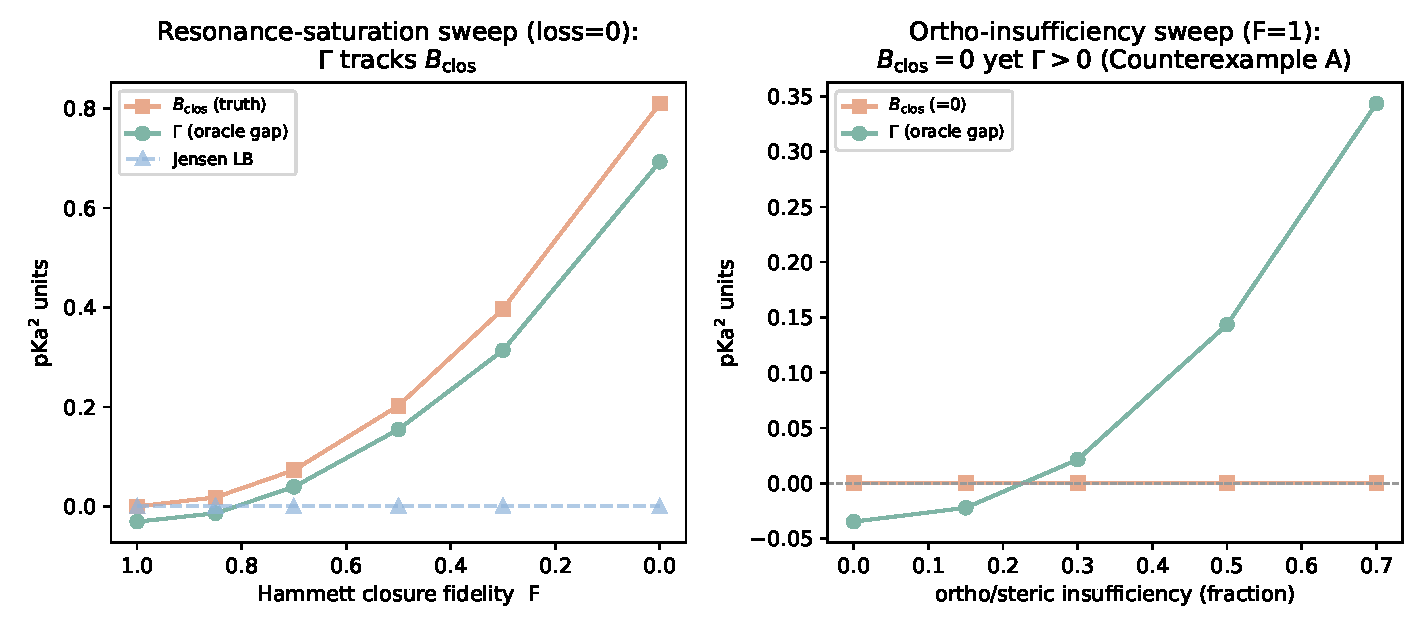
\includegraphics[width=\linewidth]{figs/fig_pka_hammett.pdf}
\caption{pKa through a Hammett LFER on a construction with known ground-truth
channels. \emph{Left:} closure fidelity varied with a sufficient intermediate; grounding gap
$\Ggap$, closure bias $\Bclos$, and the assumption-light Jensen bound. \emph{Right:} an
ortho/steric insufficiency channel varied with a \emph{well-specified} closure; $\Bclos=0$ at each
knob while $\Ggap$ rises with the insufficiency fraction, crossing zero near $0.25$.
Scope: \S\ref{sec:si-pka}.}
\label{fig:pka}
\end{figure*}
